% !TeX spellcheck = en_US
%\documentclass{beamer}
\documentclass[handout]{beamer}
\usepackage[spanish]{babel}
\usepackage[utf8]{inputenc}
\usepackage{graphicx}
\usepackage{tcolorbox}
\usepackage{color}

\usepackage{braket}
\usepackage{hyperref}
%\setbeamercolor{frametitle}{fg=white}
%\usefonttheme{structuresmallcapsserif}
\setbeamertemplate{footline}[frame number]
\setbeamerfont{footnote}{size=\tiny}

\setbeamercolor{page number in head/foot}{fg=black}

\usepackage{amsmath}
\usepackage{mhchem}
\usepackage{tikz}
\def\checkmark{\tikz\fill[scale=0.4](0,.35) -- (.25,0) -- (1,.7) -- (.25,.15) -- cycle;} 

\usepackage{default}

\usepackage[backend = bibtex, style = verbose, sorting = none, autocite = footnote]{biblatex}
\addbibresource{references.bib}

\newcommand\blfootnote[1]
{%
	\begingroup
	\renewcommand\thefootnote{}\footnote{#1}%
	\addtocounter{footnote}{-1}%
	\endgroup
}
\newcommand{\fcite}[1]{\blfootnote{\cite{#1}}}

\usetheme{Berkeley}

\begin{document}
	\begin{frame}
		\centering
		%\color{white}
		\textsc{\large Photocatalytic and electrocatalytic reduction of \ce{CO2} to methanol by the homogeneous pyridine-based systems}
		\\
		\vspace{0.5cm}
		{\scriptsize Wai Wang, Junxiao Zhang, Hui Wang, Lianjia Chen, Zhaoyong Bian}
		\\
		\vspace{3cm}
		\raggedleft Juan Barbosa \\
		\raggedleft \small Catálisis en la industria y el laboratorio
	\end{frame}

\begin{frame}{Contenidos}
	\tableofcontents
\end{frame}

\section{Introducci\'on}
\begin{frame}{Introducci\'on}
	\begin{figure}[h]
		\centering
		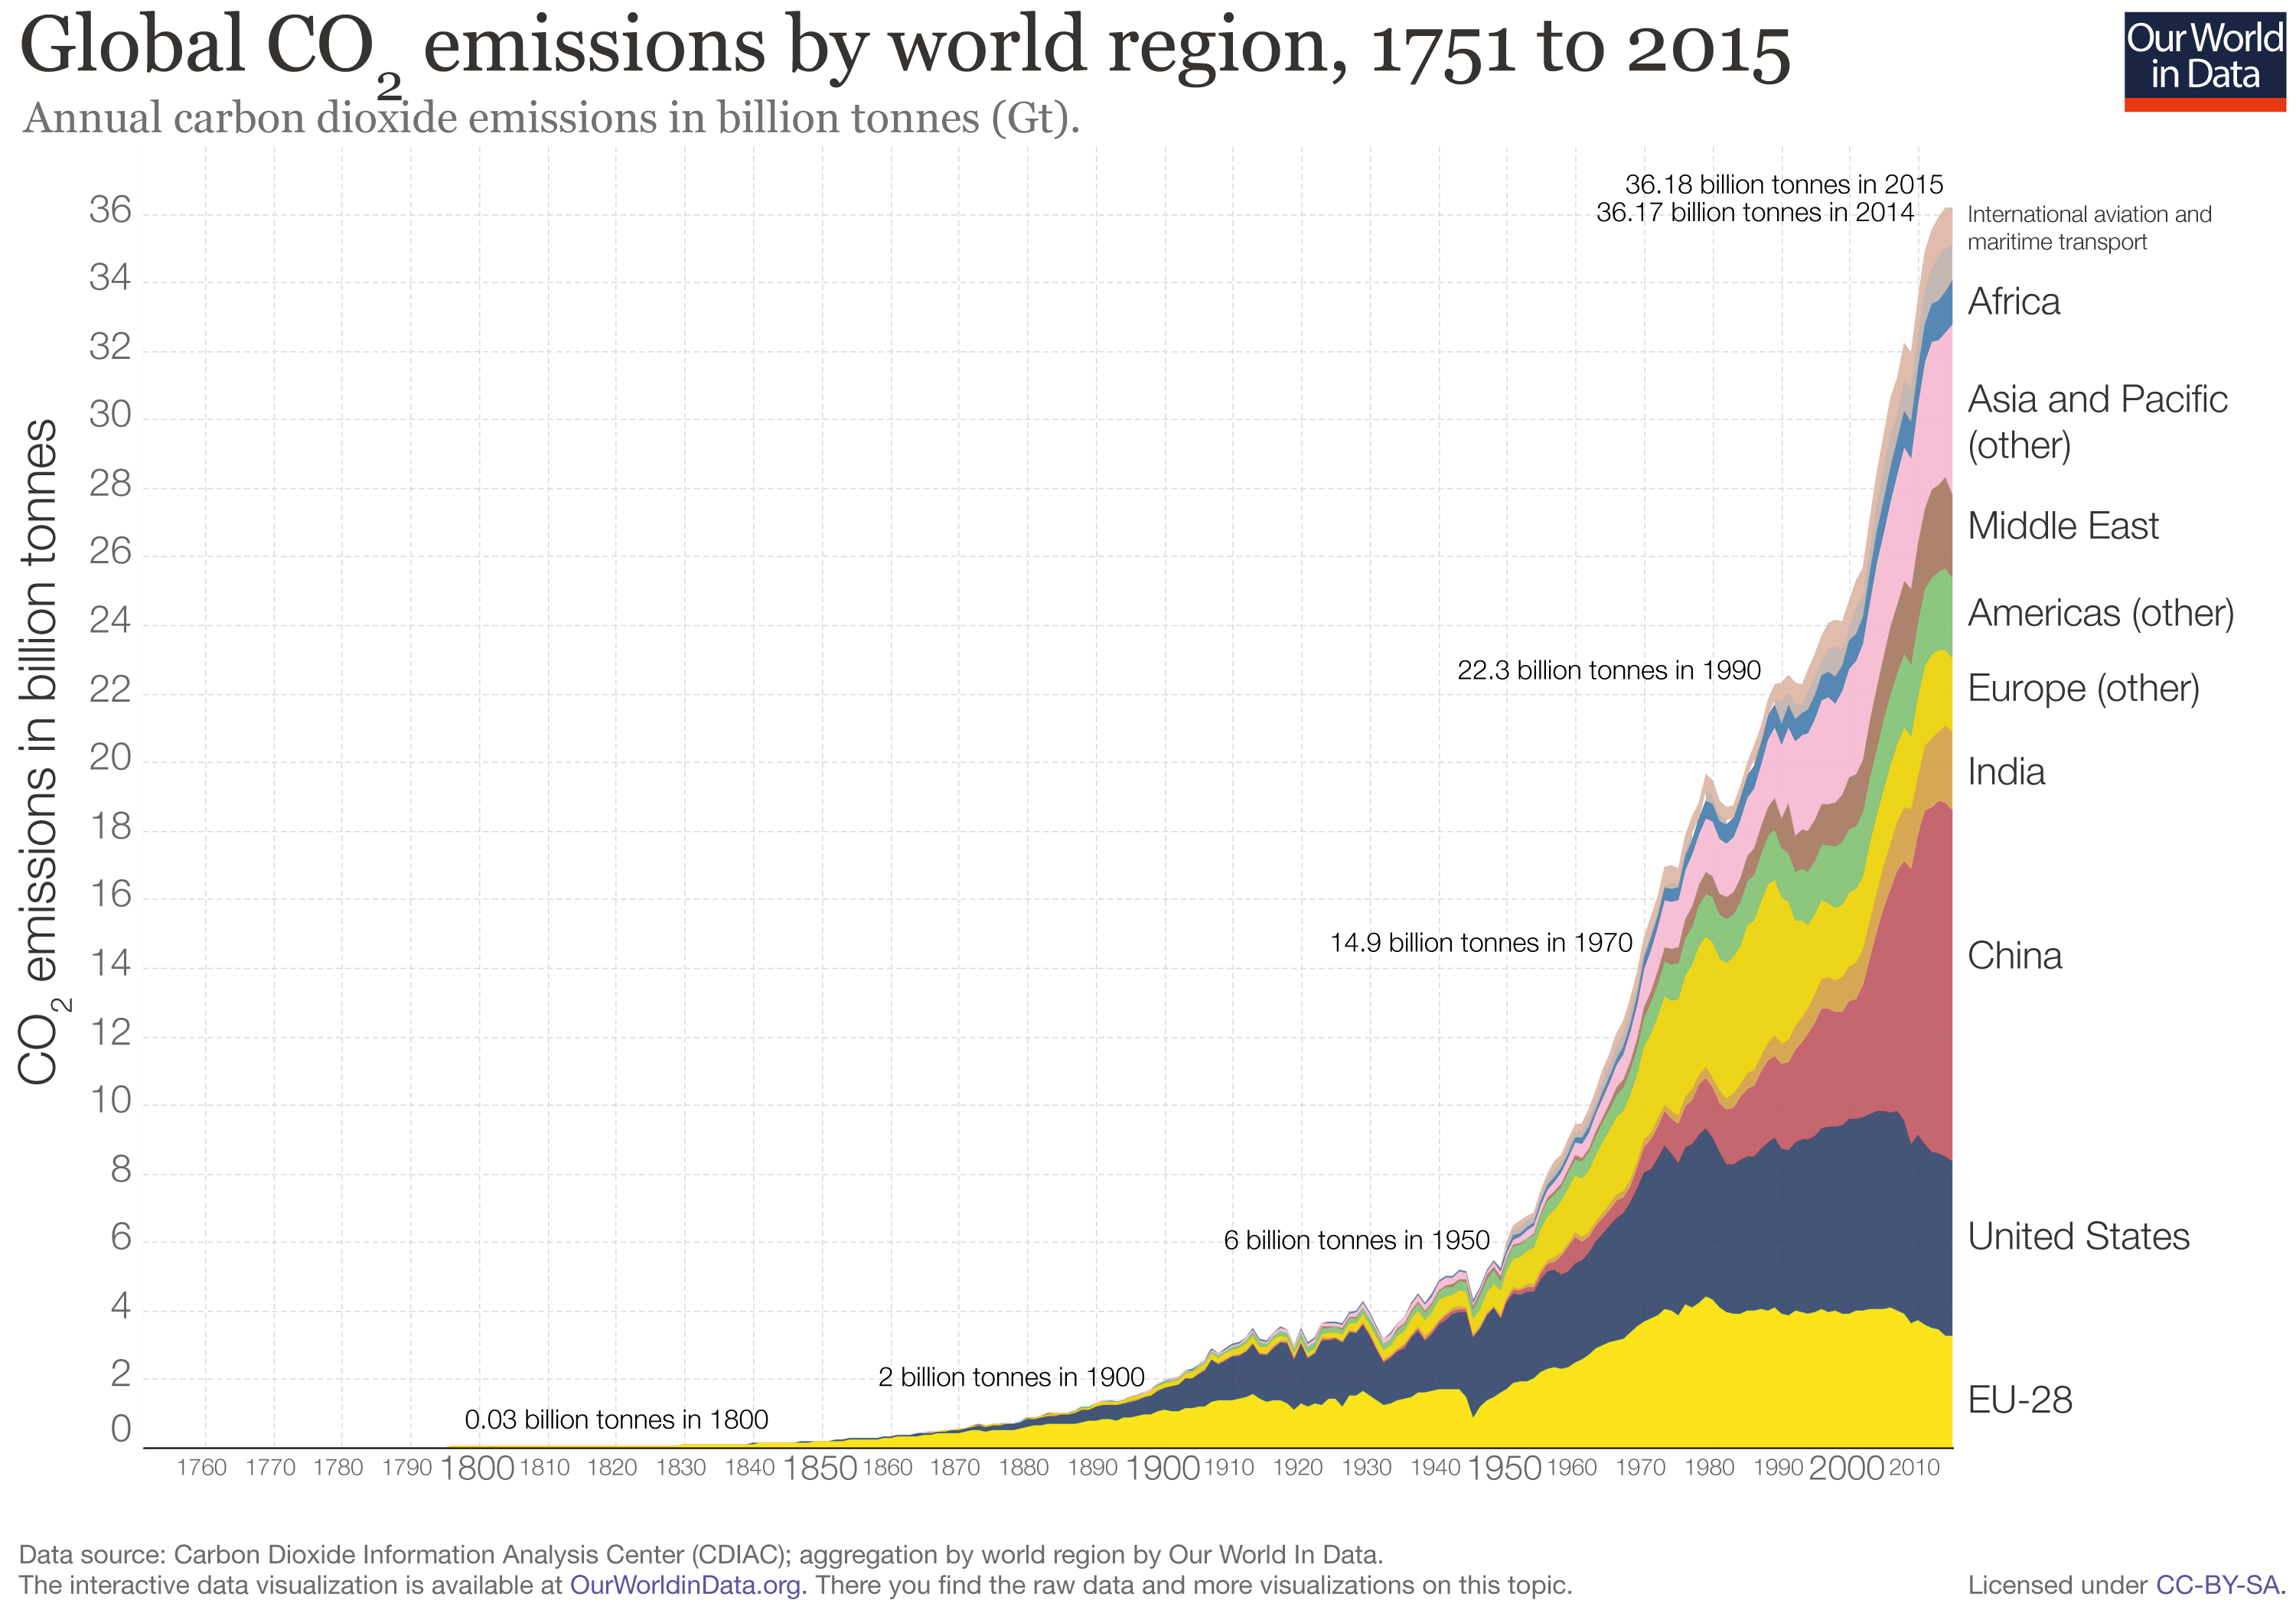
\includegraphics[width=\linewidth]{sources/CO2_emissions}
	\end{figure}
\end{frame}

\begin{frame}{Introducci\'on}
	\begin{itemize}
		\item La conversi\'on de \ce{CO2} a combustibles y energ\'ias renovables tiene efectos importantes en el medio ambiente y los sectores energ\'eticos.
		\item Dentro de estos procesos de conversi\'on se  encuentra la reducci\'on electroqu\'imica de \ce{CO2}.
		\begin{itemize}
			\item Permite obtener alquenos y alcoholes.
			\item Baja selectividad.
			\item No existe claridad sobre los mecan\'ismos.
			\item Aplicaci\'on de $V$ grandes, que inducen a altos consumos energ\'eticos.
		\end{itemize}
	\end{itemize}
\end{frame}

\begin{frame}{Introducci\'on}
	\begin{itemize}
		\item La reducci\'on fotocatal\'itica constituye una ruta atractiva, pues usa la abundancia de la radaci\'on solar para la utilizaci\'on del \ce{CO2}.
		\begin{itemize}
			\item \textbf{Fotoreducci\'on homog\'enea} usando un catalizador molecular.
			\item \textbf{Fotoreducci\'on heterog\'enea} usando semiconductores.
			\begin{itemize}
				\item \ce{TiO2} \ce{SiC} $\longrightarrow$ \ce{CO}, \ce{MeOH}, \ce{CH4}.
			\end{itemize} 
		\end{itemize}
	\end{itemize}
	\begin{figure}[h]
		\centering
		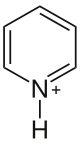
\includegraphics[width=0.1\linewidth]{sources/pyridinium}
	\end{figure}
	Ion piridinio logra hasta 30 \% de rendimiento Far\'adico para metanol en electrodos de paladio hidrogenados.
\end{frame}

\begin{frame}{Introducci\'on}
	\begin{figure}[h]
		\centering
		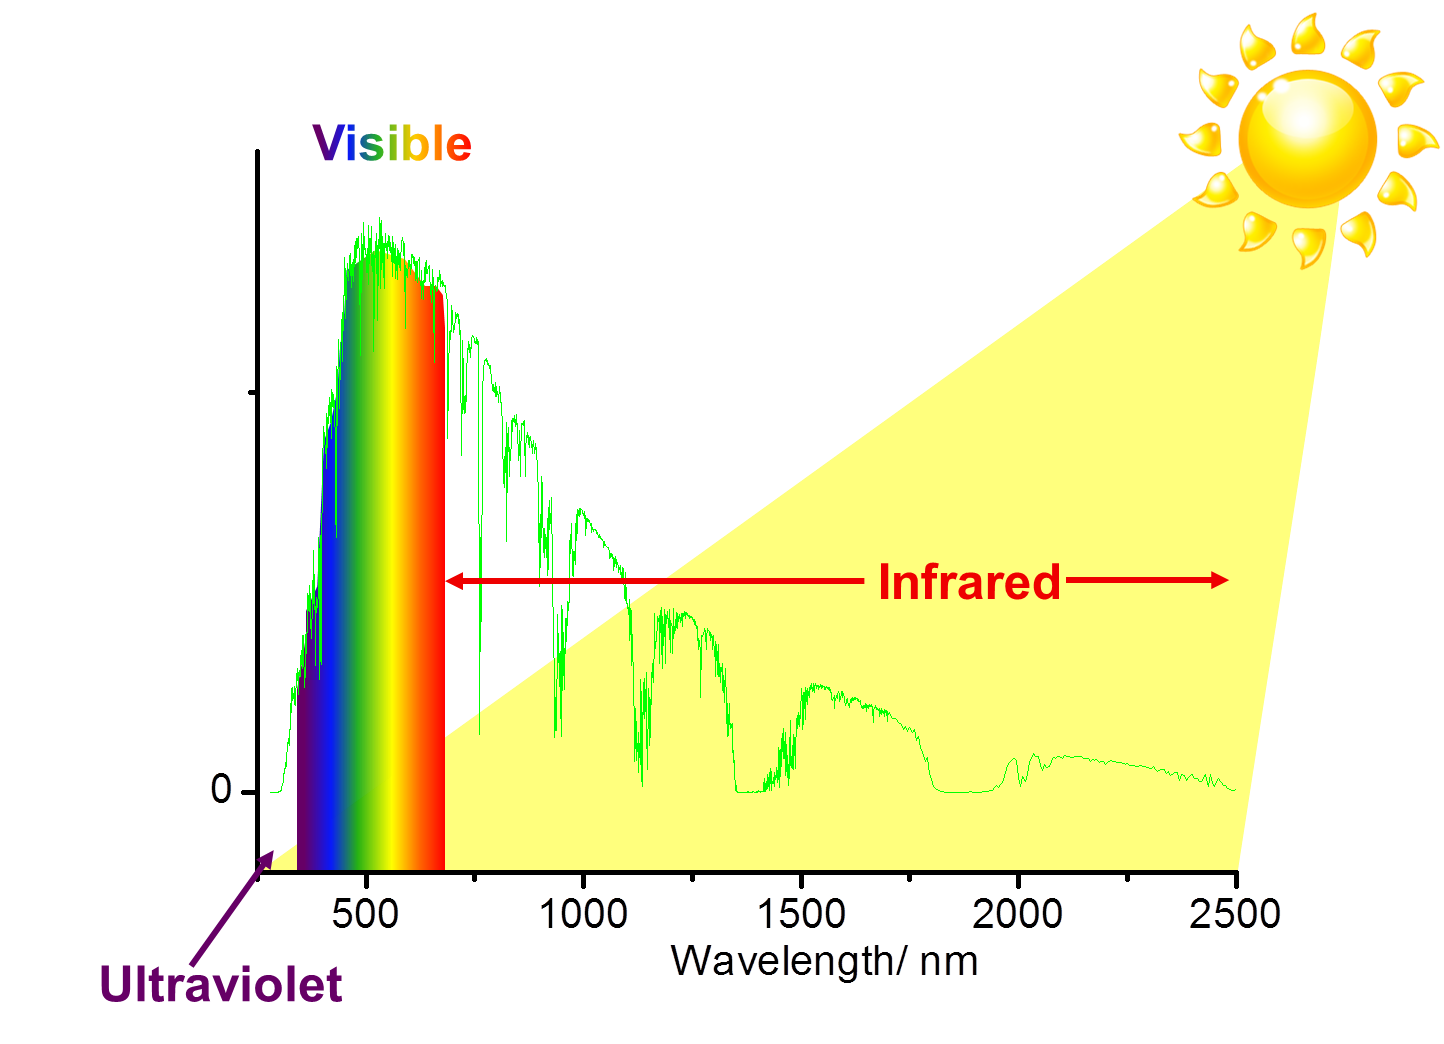
\includegraphics[width=0.8\linewidth]{sources/spectrum}
	\end{figure}
	\begin{itemize}
		\item Complejos de renio absorben mayormente en el UV.
		\item Bajo TON, y selectividad.
	\end{itemize}
\end{frame}

\section{Procedimiento experimental}
\begin{frame}{Procedimiento experimental}
	Preparaci\'on de \ce{[Ru(phen)_3](PF6)2}.
	\begin{itemize}
		\item Reflujo por 8 horas.
		\begin{equation*}
			\ce{EtOH}(l) + 
			\begin{cases}
				\ce{RuCl3} &  \text{(0.42 g, 2 mmol)} \\
				\ce{1,10-fenantrolina} & \text{(1.09 g, 6 mmol)}
			\end{cases}
			+ \ce{N2(g)}
		\end{equation*}
		\item Posteriormente se adiciona \ce{NH4PH6} (3.26 g, 20 mmol).
		\item El s\'olido se filtra y se seca al vac\'io.
	\end{itemize}
	\begin{figure}[h]
		\centering
		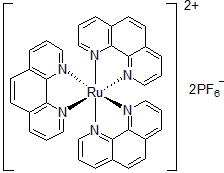
\includegraphics[width=0.3\linewidth]{sources/ru}
	\end{figure}
\end{frame}

\begin{frame}{Procedimiento experimental}
	\footnotesize
	\begin{columns}
		\begin{column}{0.2\linewidth}
			\textbf{$^1$HRMN}
			\begin{figure}[h]
				\centering
				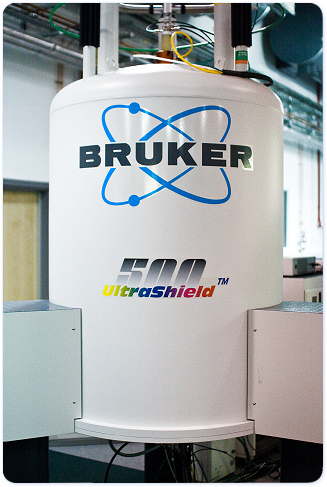
\includegraphics[width=\textwidth]{sources/bruker}
			\end{figure}
		\end{column}
		\begin{column}{0.25\linewidth}
			\textbf{Absorci\'on UV-vis}
			\begin{figure}[h]
				\centering
				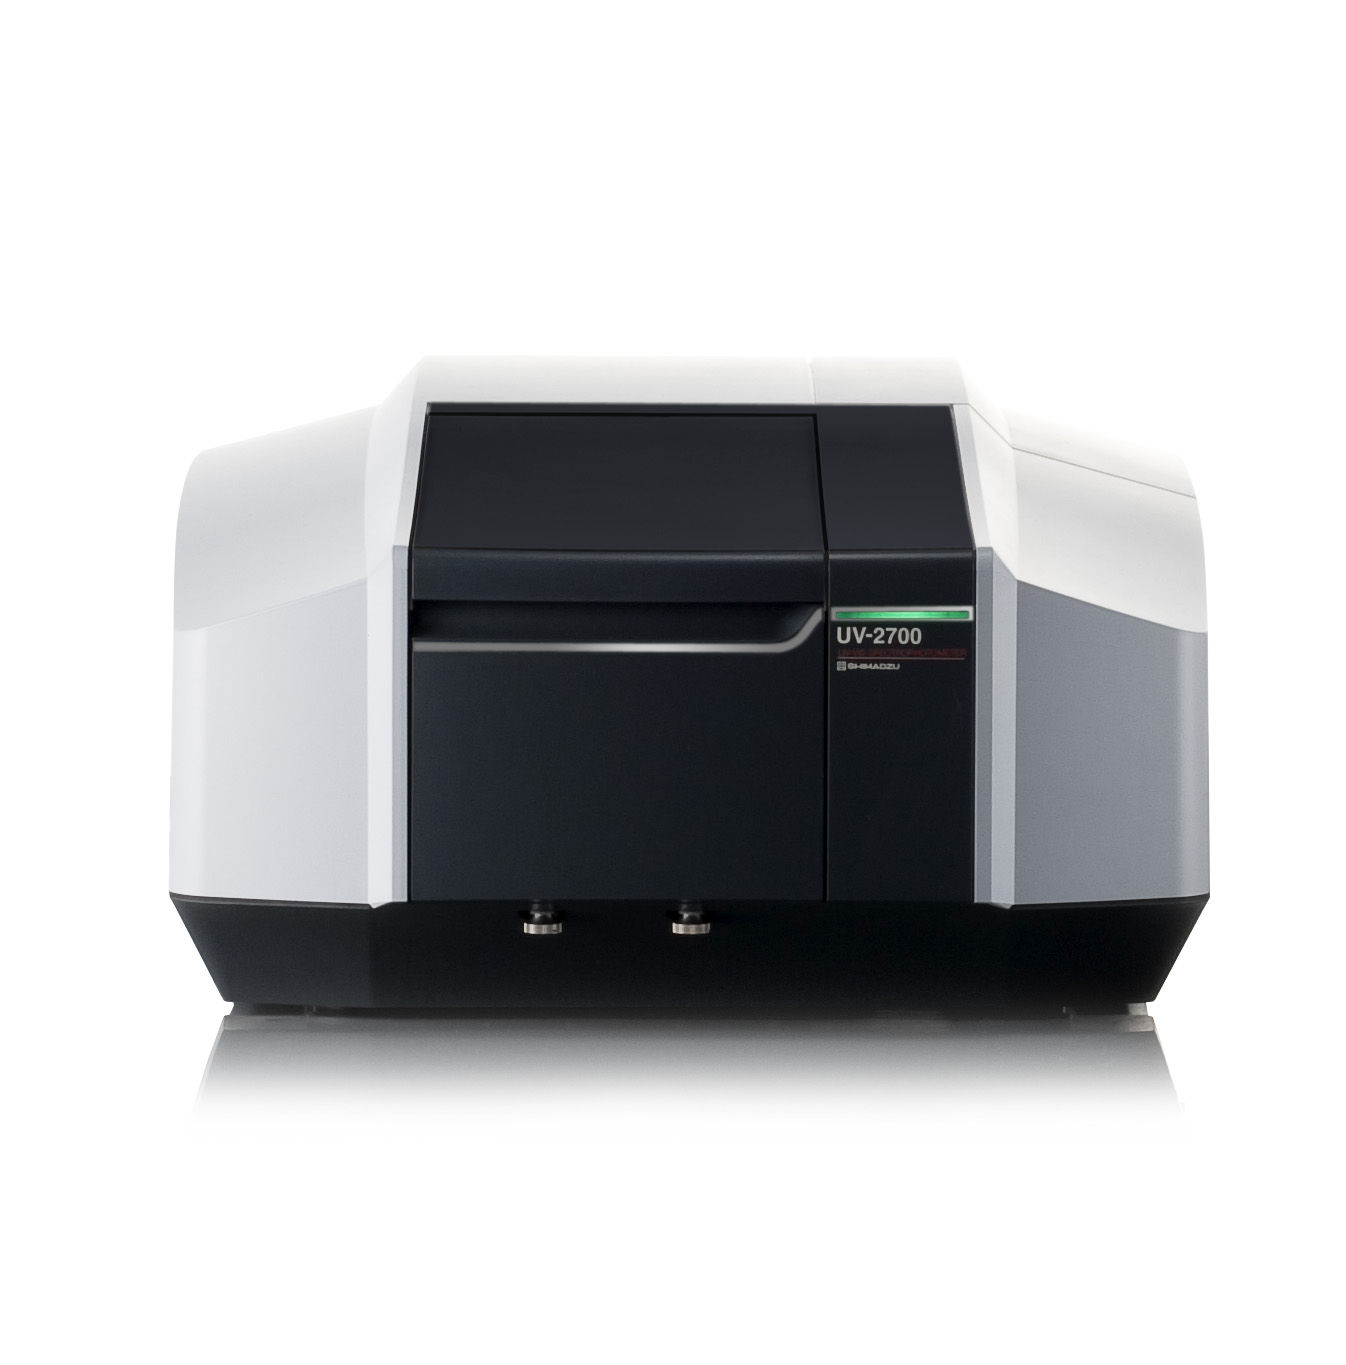
\includegraphics[width=\textwidth]{sources/uvviseq}
			\end{figure}
			\tiny
			\begin{itemize}
				\item Celdas de cuarzo.
				\item S = \ce{CH3CN} : \ce{H2O}
				\item C = 0.02 mM.
				\item 200 - 800 nm.
			\end{itemize}
		\end{column}
		\begin{column}{0.25\linewidth}
			\textbf{Fotoluminiscencia}
			\begin{figure}[h]
				\centering
				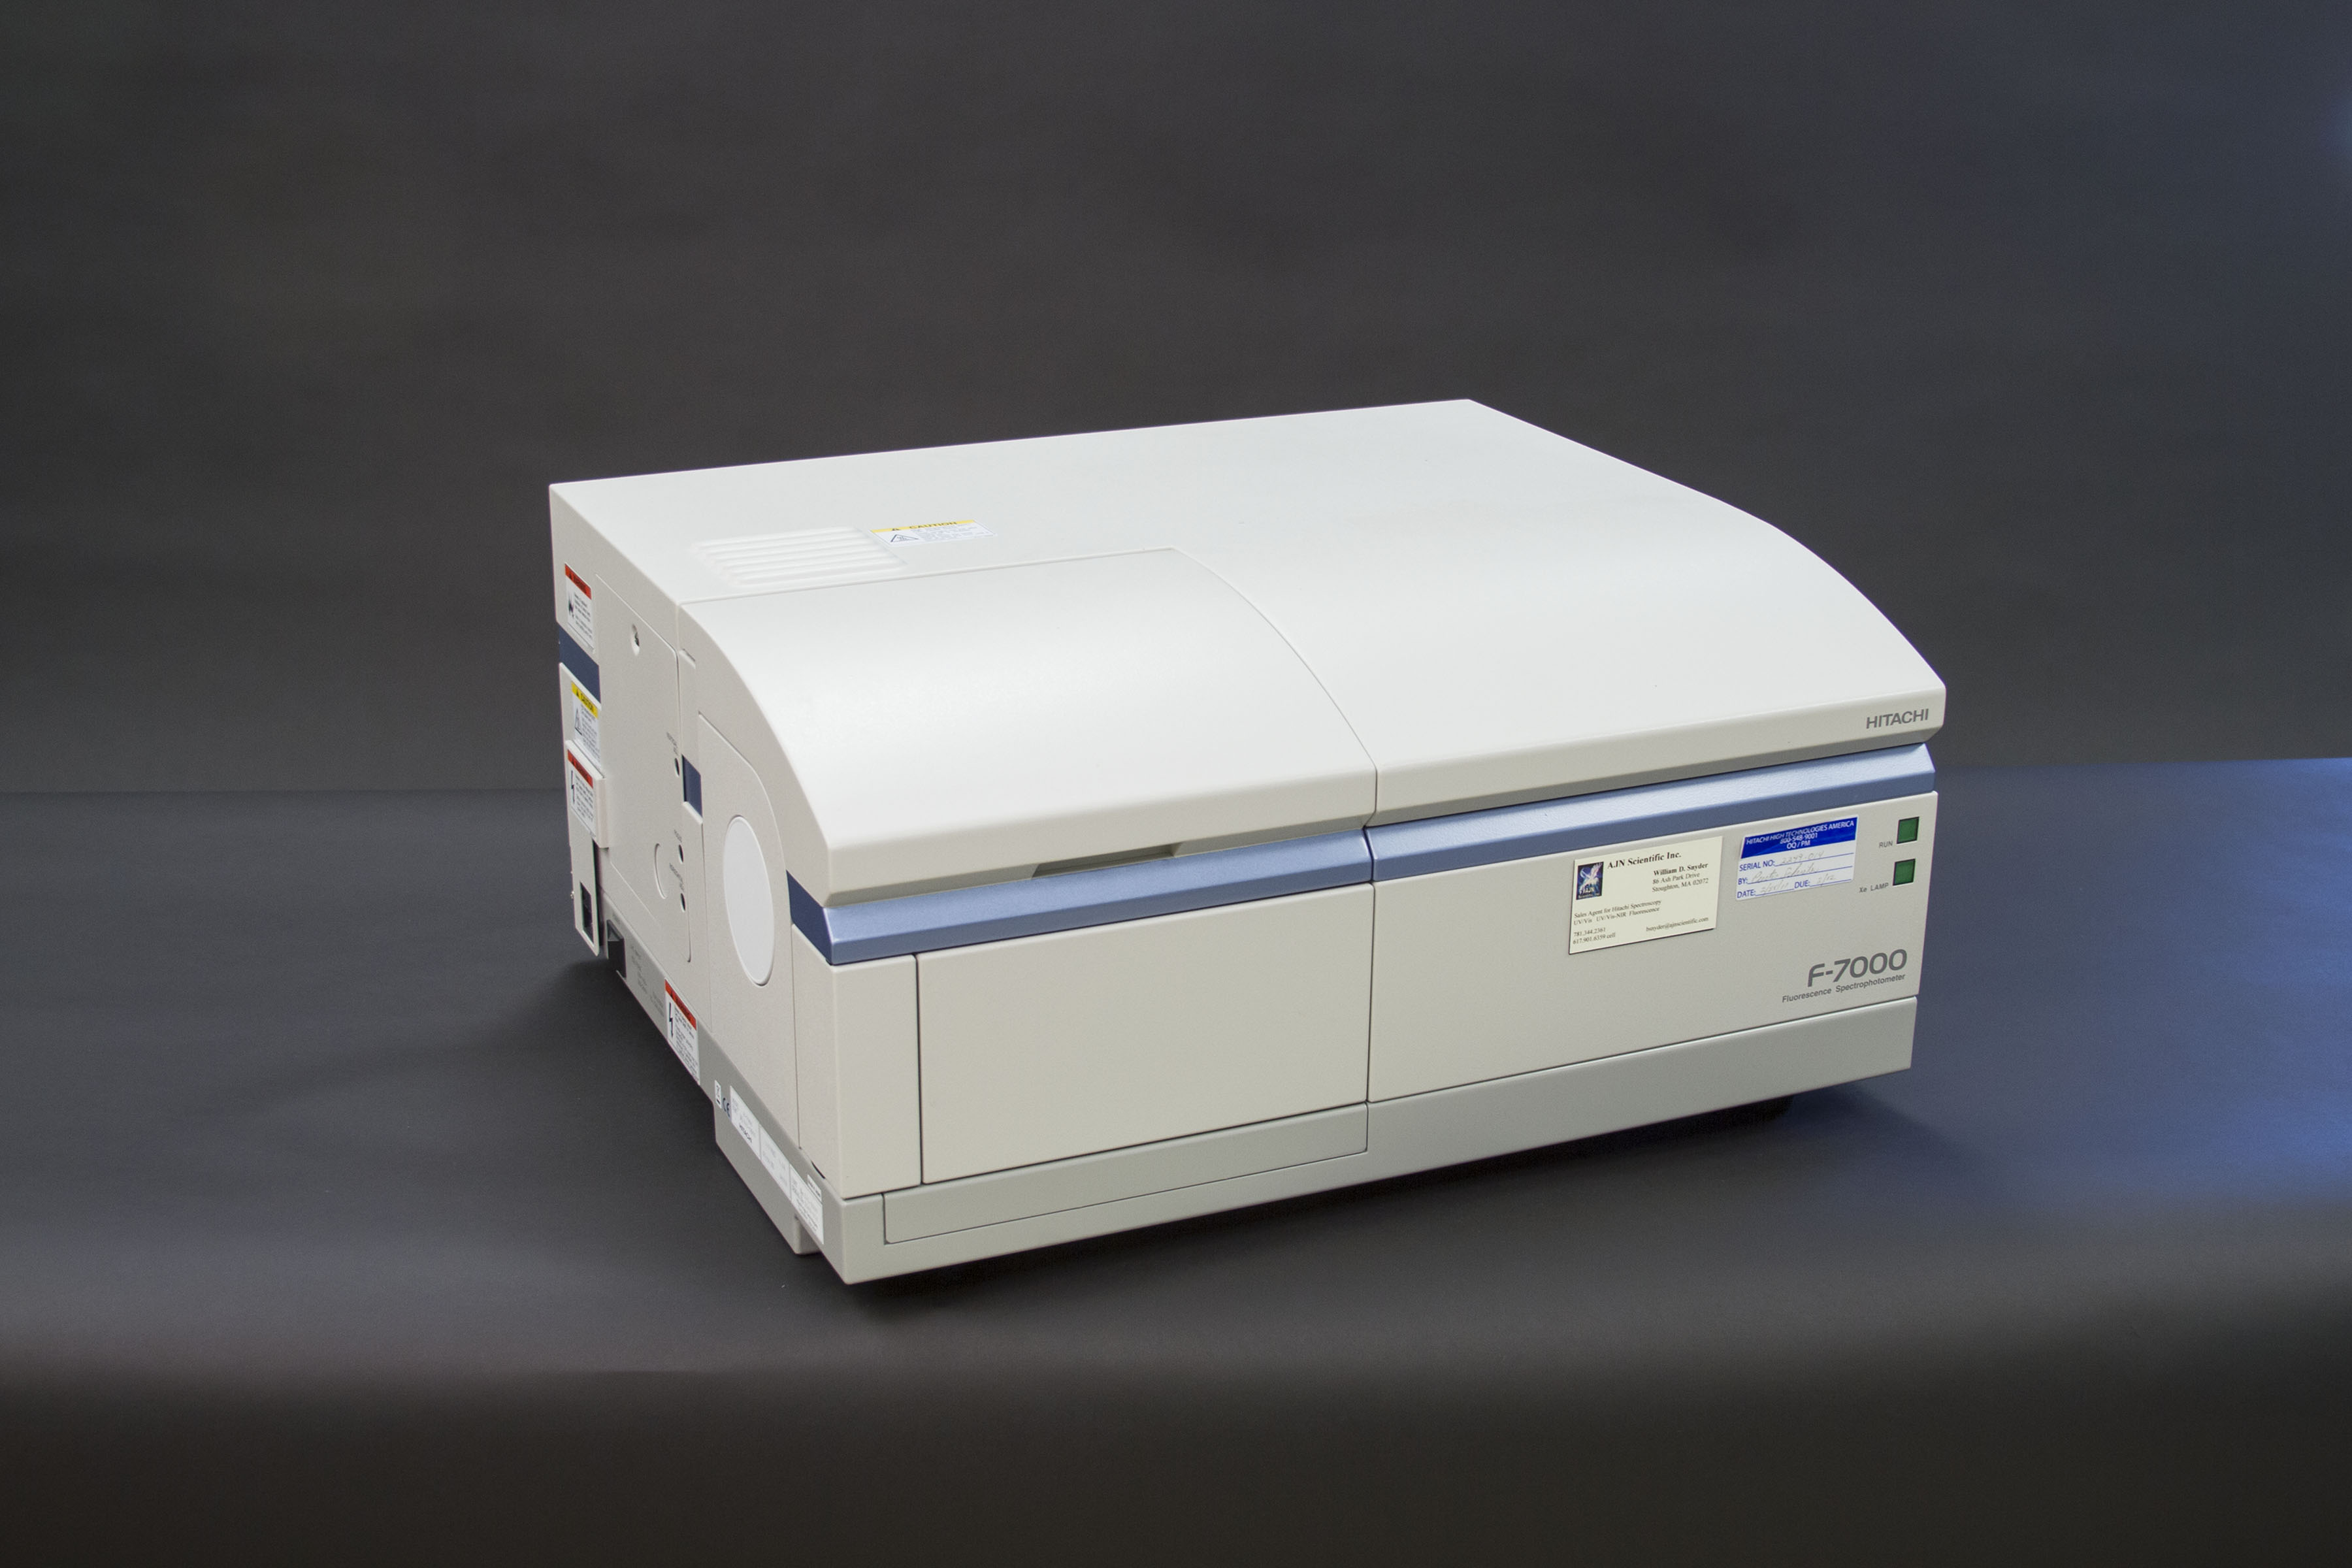
\includegraphics[width=\textwidth]{sources/fluorescence}
			\end{figure}
			\tiny
			\begin{itemize}
				\item Celdas de cuarzo.
				\item S = \ce{CH3CN} : \ce{H2O}
				\item C = 0.02 mM.
				\item 500 - 800 nm.
			\end{itemize}
		\end{column}
		\begin{column}{0.2\linewidth}
			\textbf{Electroqu\'imica}
			\begin{figure}[h]
				\centering
				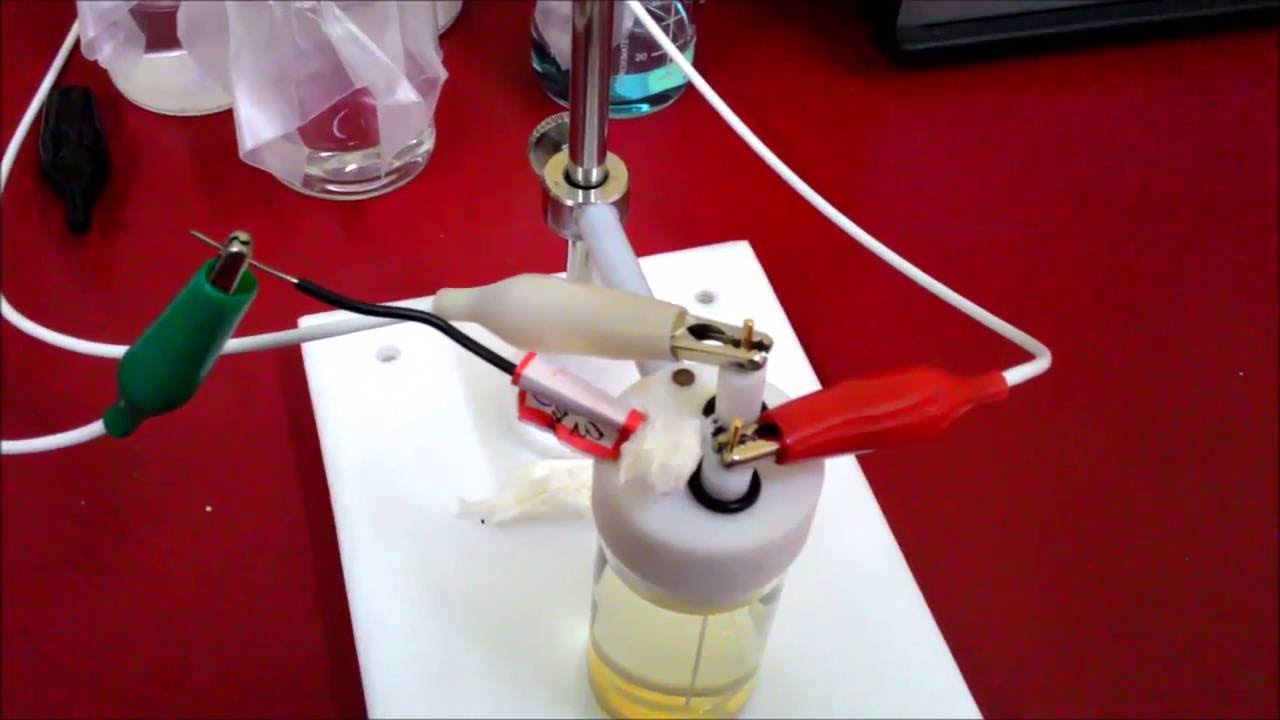
\includegraphics[width=\textwidth]{sources/electrical}
			\end{figure}
			\tiny
			\begin{itemize}
				\item WE: Pt
				\item RE: Ag/AgCl en KCl
				\item CE: Pt
			\end{itemize}
		\end{column}
	\end{columns}
	\vspace{1cm}
%	KCl y \ce{(CH3CH2CH2CH2)4N(PF6)} son usados como electrolitos. Las soluciones son burbujeadas con \ce{N2} y \ce{CO2} por 40 minutos.
\end{frame}


\begin{frame}{Procedimiento experimental}
	En 25 mL de acetonitrilo.
	\begin{columns}
		\begin{column}{0.6\linewidth}
			\begin{figure}[h]
				\centering
				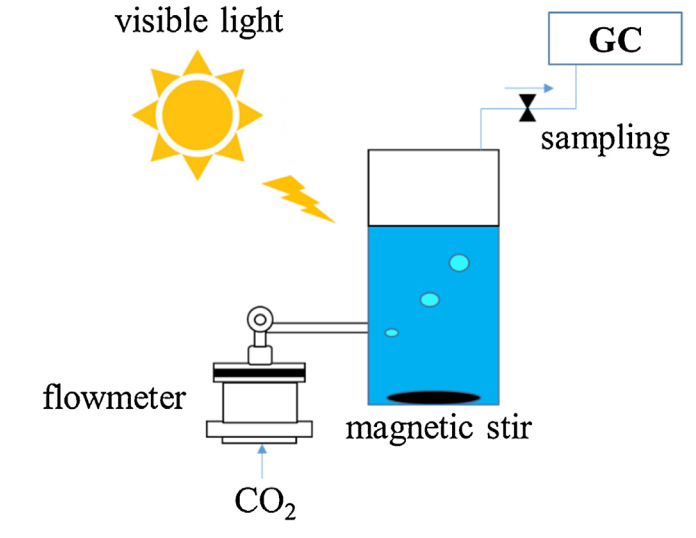
\includegraphics[width=\textwidth]{sources/reactor}
			\end{figure}
		\end{column}
		\begin{column}{0.4\linewidth}
			\footnotesize
			\begin{itemize}
				\item \ce{[Ru(phen)3](PF6)2} (0.020 mM)
				\item Piridina (50 mM)
%				\item KCl (0.1 mM)
				\item \'Acido asc\'orbico (0.2 mM)
			\end{itemize}
			\vspace{0.5cm}
			\begin{itemize}
				\item pH 4, 5, 6
				\item Lampara de Xe (500 W, $\lambda >$ 420 nm)
				\item Agitaci\'on por 1-6 horas.
			\end{itemize}
		\end{column}
	\end{columns}
\end{frame}

\section{Resultados y discusi\'on}
\begin{frame}{Resultados y discusi\'on}
	\begin{itemize}
		\item $^1$HRMN para el fotosensibilizador (\ce{[Ru(phen)3](PF6)2}).
	\end{itemize}
	\begin{figure}[h]
		\centering
		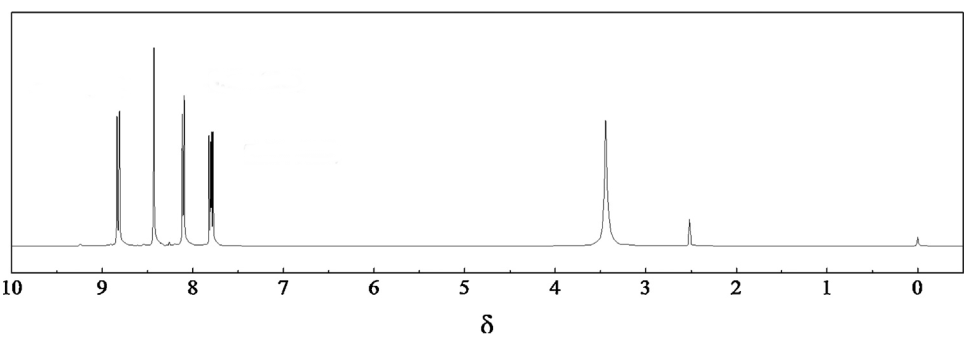
\includegraphics[width=\linewidth]{sources/hnmr}
	\end{figure}
	$^1$HNMR (500 MHz, \ce{CDCl3}): $\delta$ 8.79 (d, J = 8.0 Hz, 6H), 8.40 (s, 6H), 8.11 (d, J = 4.0 Hz,
	6H), 7.80 (m, 6H).
\end{frame}

\begin{frame}{Resultados y discusi\'on}
	\begin{columns}
		\begin{column}{0.4\textwidth}
			\begin{figure}[h]
				\centering
				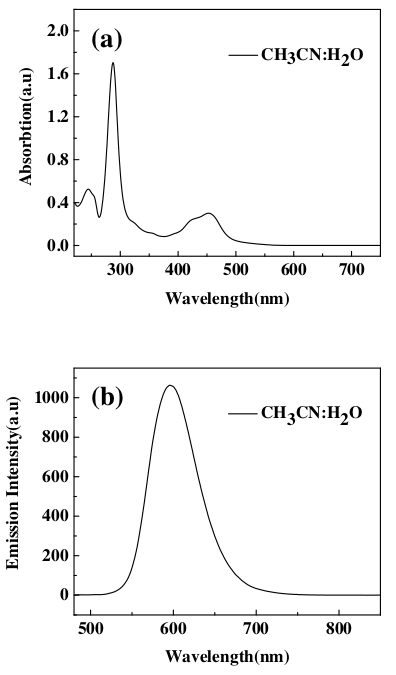
\includegraphics[width=\linewidth]{sources/spectra}
			\end{figure}
		\end{column}
		\begin{column}{0.6\textwidth}
			\begin{itemize}
				\item Banda de absorci\'on por transferencia de carga metal ligando en 451 nm.
				\item En la regi\'on UV, se tienen transiciones $\pi$-$\pi^*$ en la fenantrolina.
				\item El fotosensibilizador presenta emisi\'on en 600 nm.
			\end{itemize}
		\end{column}
	\end{columns}
\end{frame}

\begin{frame}{Resultados y discusi\'on}
	\begin{columns}
		\footnotesize
		\begin{column}{0.6\textwidth}
			\begin{itemize}
				\item Potencial de oxidaci\'on de la p\'erdida de un $e^-$ por \ce{[Ru(phen)3]^{2+}} en $1.2$ V.
				\item Potenciales de reducci\'on en $-1.38$ V, $-1.64$ V, $-1.85$ V.
			\end{itemize}
		\tiny
		\vspace{0.5cm}
		\begin{equation}
			\ce{[Ru(phen)3]^{2+} - e^- -> [Ru(phen)3]^{3+}}
		\end{equation}
		\begin{equation}
			\ce{[Ru(phen)3]^{2+} + e^- -> [Ru(phen)2(phen^-)]^{1+}}
		\end{equation}
		\begin{equation}
			\ce{[Ru(phen)2(phen^-)]^{1+} + e^- -> [Ru(phen)(phen^-)2]^{\bullet}}
		\end{equation}
		\begin{equation}
			\ce{[Ru(phen)(phen^-)2]^{\bullet} + e^- -> [Ru(phen^-)3]^{-}}
		\end{equation}		
		
		\end{column}
		\begin{column}{0.4\textwidth}
			\begin{figure}[h]
				\centering
				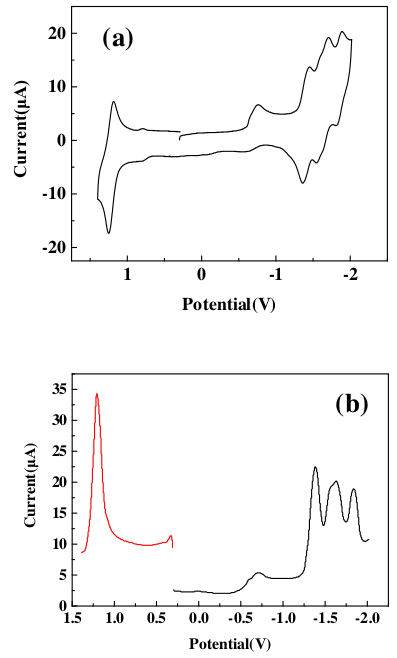
\includegraphics[width=\linewidth]{sources/cv}
			\end{figure}
		\end{column}
	\end{columns}
\end{frame}

\begin{frame}{Resultados y discusi\'on}
	\begin{columns}
		\begin{column}{0.4\textwidth}
			\begin{figure}[h]
				\centering
				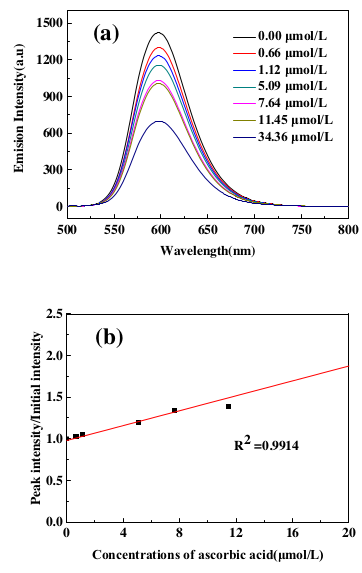
\includegraphics[width=\linewidth]{sources/uv}
			\end{figure}
		\end{column}
		\begin{column}{0.6\textwidth}
			\'Acido asc\'orbico como desactivante de la fluorescencia.
			\begin{itemize}
				\item La emisi\'on del complejo se redujo con el aumento de la concentraci\'on del \'acido.
				\item La desactivaci\'on del complejo permite la obtenci\'on de especies reducidas que transfieren electrones al \ce{CO2}. 
			\end{itemize}
		\end{column}
	\end{columns}
\end{frame}

\begin{frame}{Resultados y discusi\'on}
	\begin{figure}[h]
		\centering
		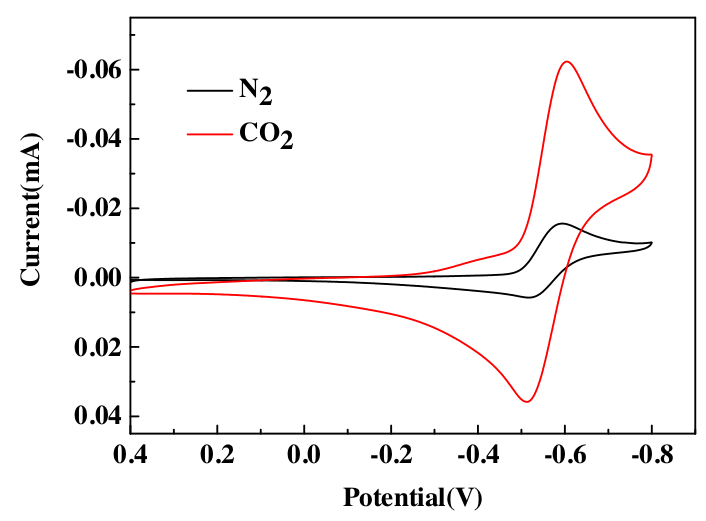
\includegraphics[width=0.7\linewidth]{sources/CO2N2}
	\end{figure}
	El pico de reducci\'on es mayor para \ce{CO2}, existe una reacci\'on entre el catalizador de piridina y el \ce{CO2}.
\end{frame}

\begin{frame}{Resultados y discusi\'on}
	\begin{columns}
		\begin{column}{0.4\textwidth}
			\begin{figure}[h]
				\centering
				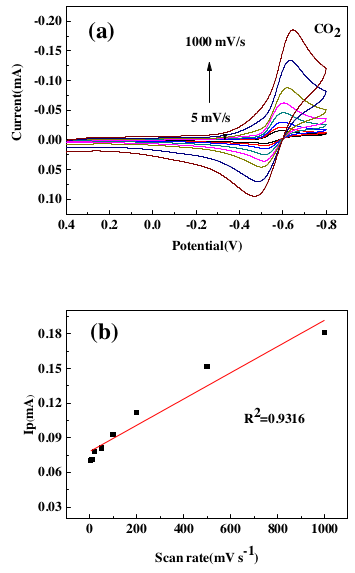
\includegraphics[width=\linewidth]{sources/scan}
			\end{figure}
		\end{column}
		\begin{column}{0.6\textwidth}
			Usando la ecuaci\'on de Cottrell:
			\begin{equation}
				I = \dfrac{nFAc_j^0\sqrt{D_j}}{\sqrt{\pi}t^\alpha} = kt^{-\alpha}
			\end{equation}
			\begin{figure}[h]
				\centering
				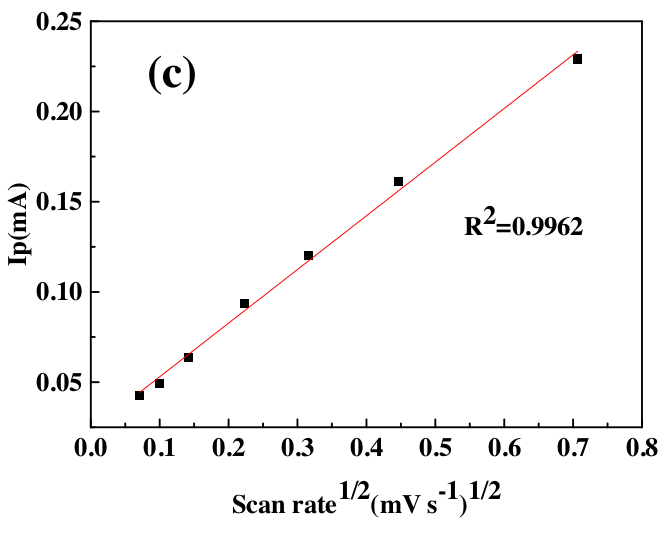
\includegraphics[width=0.6\linewidth]{sources/scan2}
			\end{figure}
			La velocidad de reacci\'on est\'a determinada por el \ce{CO2} en soluci\'on, no por el n\'umero de sitios activos.
		\end{column}
	\end{columns}
\end{frame}

\begin{frame}{Resultados y discusi\'on}
	\begin{columns}
		\begin{column}{0.5\textwidth}
			\begin{itemize}
				\item pH $\propto$ 1/\ce{[PyH+]}
				\item Potenciales de reducci\'on constantes a pH = \{4, 5\}.
			\end{itemize}
		\end{column}
		\begin{column}{0.5\textwidth}
			\begin{figure}[h]
				\centering
				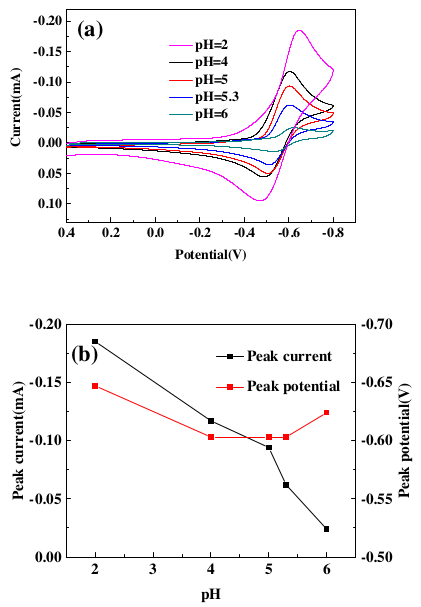
\includegraphics[width=\linewidth]{sources/pH}
			\end{figure}
		\end{column}
	\end{columns}
\end{frame}

\begin{frame}{Resultados y discusi\'on}
	\begin{columns}
		\begin{column}{0.4\textwidth}
			\begin{figure}[h]
				\centering
				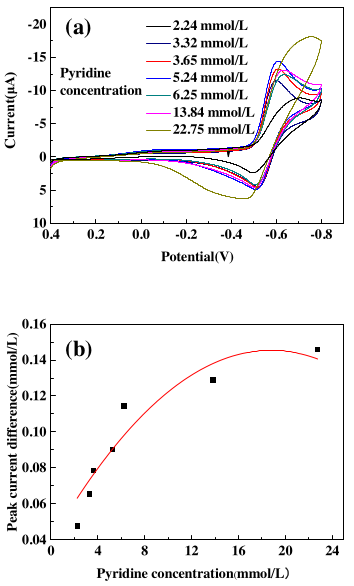
\includegraphics[width=\linewidth]{sources/concentration}
			\end{figure}
		\end{column}
		\begin{column}{0.6\textwidth}
			\begin{itemize}
				\item La intensidad del pico de reducci\'on aument\'o significativamente con el aumento de piridina.
				\item La diferencia aument\'o hasta alcanzar una plataforma.
				\item La reacci\'on est\'a limitada a la concentraci\'on de la piridina.
			\end{itemize}
		\end{column}
	\end{columns}
\end{frame}

\begin{frame}{Resultados y discusi\'on}
	\begin{figure}[h]
		\centering
		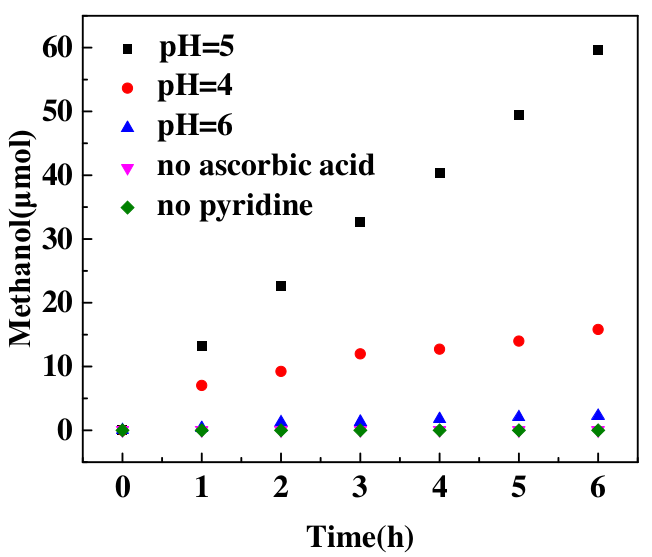
\includegraphics[width=0.5\linewidth]{sources/pHt}
	\end{figure}
	El pH fue determinado como el factor m\'as importante en la reacci\'on catal\'itica.
\end{frame}

\begin{frame}{Resultados y discusi\'on}
	\begin{itemize}
		\item El cati\'on piridinio (\ce{PyH+}) se reduce al radical ($\ce{PyH^{\bullet}}$) con un electr\'on del \ce{[Ru(phen)3](PF6)2}.
		\item La esp\'ecie $\ce{PyH^{\bullet}}$ reacciona con \ce{CO2} para formar $\ce{PyCOOH^{\bullet}}$.
	\end{itemize}
	\begin{figure}[h]
		\centering
		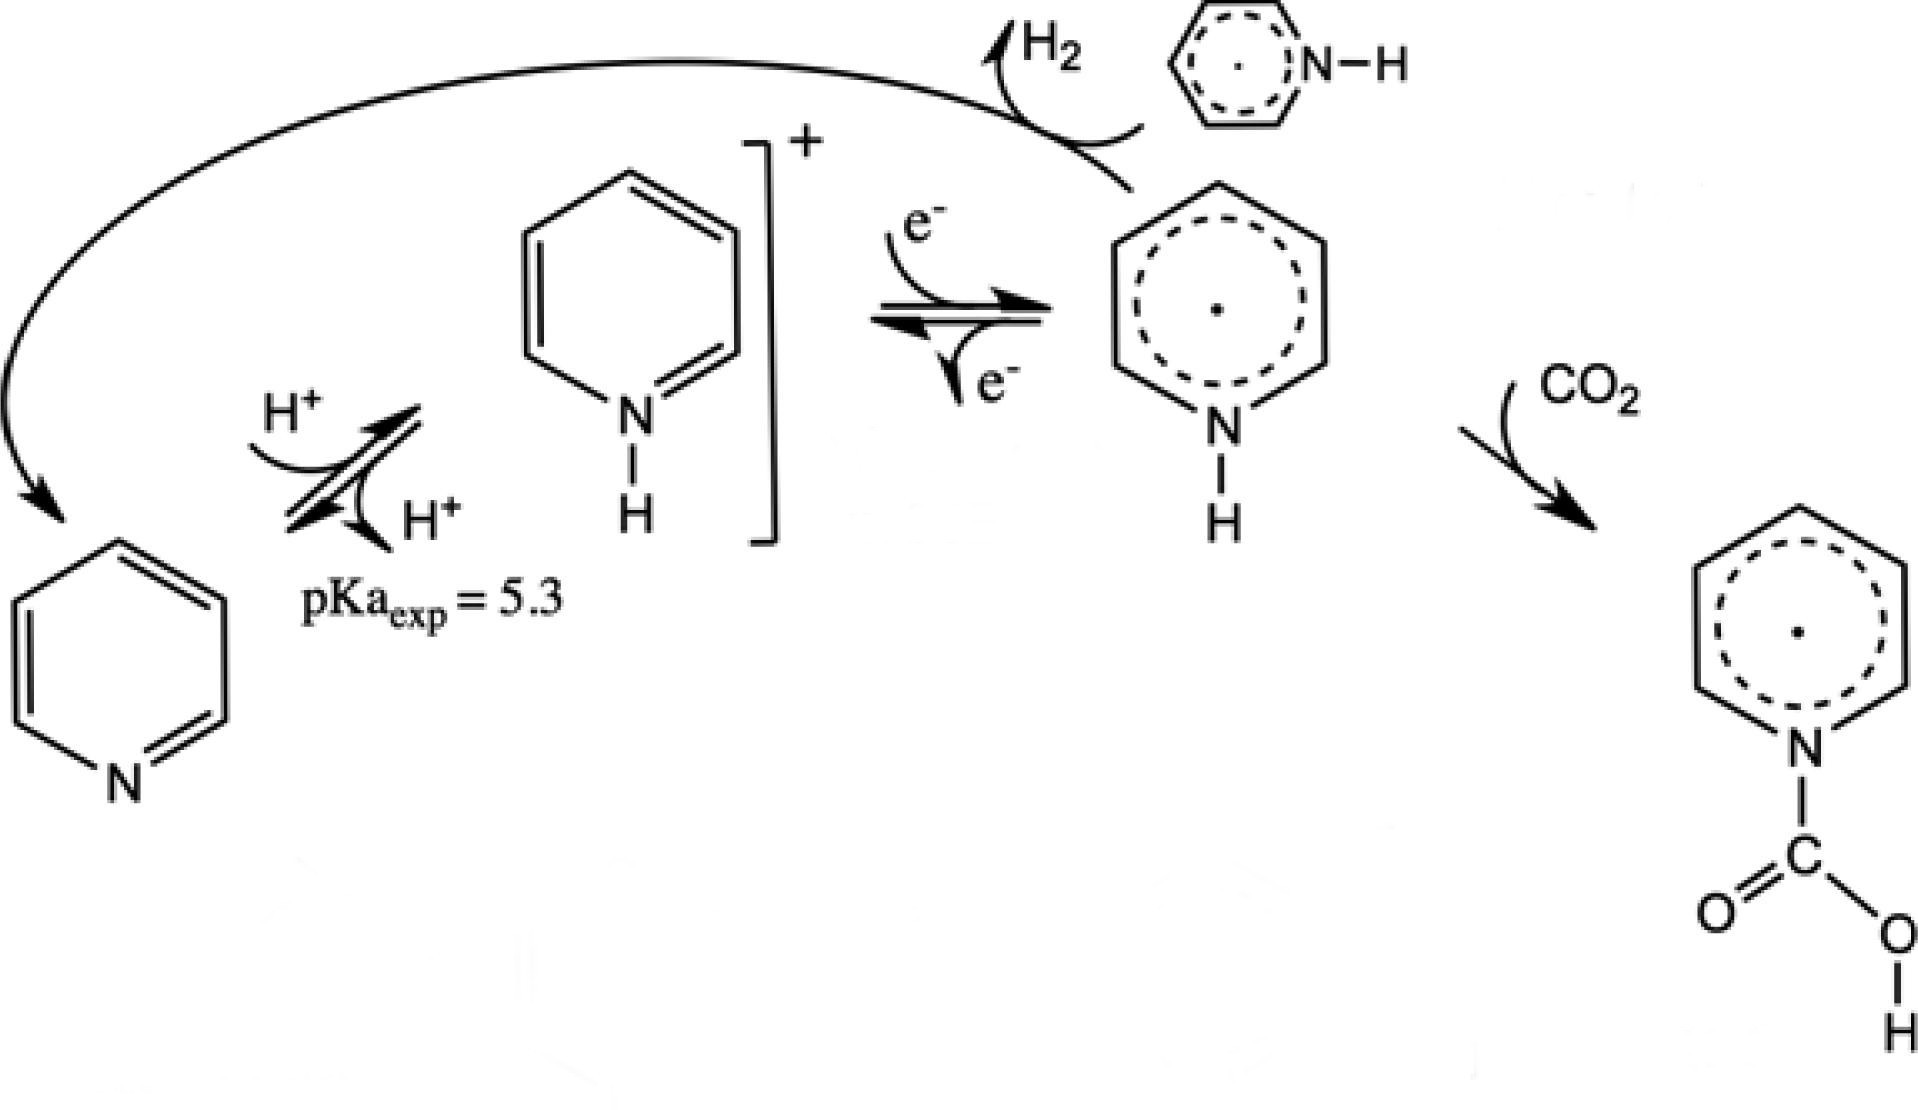
\includegraphics[width=0.6\linewidth]{sources/mechanism}
	\end{figure}
	\fcite{lim2012mechanism}
\end{frame}

\section{Conclusiones}
\begin{frame}{Conclusiones}
	\begin{itemize}
		\item \ce{[Ru(phen)_3](PF6)2} es un buen fotosensibilizador (400 - 500 nm) en el rango visible.
		\item El electr\'on generado por el fotosensibilizador antes de que tenga lugar una recombinaci\'on.
		\item Cuando el \# de electrones y el \# de sitios activos sean iguales. Se tienen las condiciones \'optimas.
		\item Cuando la concentraci\'on de piridina es mayor a 6.35 mM, existe otra reacci\'on redox.
		\begin{block}{}
			Las mejores condiciones son: \ce{[Py]}2-6mM, y pH = 5.
		\end{block}
	\end{itemize}
\end{frame}

\end{document}